\documentclass[brazil,hardcopy,openany,a5paper]{ufscthesis}
\usepackage[brazil]{babel}
\usepackage{amsfonts, amsmath, amsthm, amsbsy,amssymb,bm,mathtools} % For math fonts, symbols and environments %
\usepackage{graphicx} 		% Required for including images
\usepackage{transparent}	% may be required for inkscape pdf figures (http://bit.ly/18i5Oga)
\usepackage{listings}
\usepackage[abnt-emphasize=bf]{abntex2cite}
\usepackage{caption}
\usepackage{multirow}
\usepackage{lscape}
\usepackage[T1]{fontenc}
\sloppy
\usepackage{siunitx}
\usepackage{nameref}
\usepackage{float}

\newcommand{\source}[1]{\small \caption*{Fonte: {#1}} } % Criar fonte embaixo da figura

\newsubfloat{figure}		% Allow subfloats in figure environment (http://bit.ly/1C20NAj)
\graphicspath{{figures/}} 	% Location of the graphics files

\usepackage{siunitx} % units package
\let\DeclareUSUnit\DeclareSIUnit
\let\US\SI
\let\us\si
\DeclareUSUnit\inch{in}
\sisetup{detect-all}  %it may be necessary to load it after loading the font package

\citebrackets[]

%----------------------------------------------------------------------
% Comandos criados pelo usuário
\newcommand{\afazer}[1]{{\color{red}{#1}}} % Para destacar uma parte a ser trabalhada
\DeclareMathOperator*{\argmin}{\arg\!\min}
\DeclareMathOperator*{\argmax}{\arg\!\max}

%----------------------------------------------------------------------
% Identificadores do trabalho
% Usados para preencher os elementos pré-textuais
\instituicao[a]{Universidade Federal de Santa Catarina} % Opcional
\departamento[a]{Biblioteca Universitária}
\programa[o]{Programa de Pós-Graduação em Engenharia Civil} 
\curso{Engenharia de Engenharia Civil}
\documento[a]{Dissertação} % [o] para dissertação e trabalho de conclusão de curso [a] para tese
\grau{Mestre} % doutor, mestre, engenheiro, etc.
\titulo{PREDIÇÃO DE CONFORTO TÉRMICO EM ESCRITÓRIOS VENTILADOS NATURALMENTE POR MEIO DE REDES NEURAIS ARTIFICIAIS}
\subtitulo{} % Opcional
\autor{Marcelo Salles Olinger}
\local{Florianópolis} % Opcional (Florianópolis é o padrão)
\data{28}{Fevereiro}{2019}
\orientador[Universidade Federal de Santa Catarina]{Profa. Ana Paula Melo, Dra.}

\begin{document}
	
	\frontmatter
	\folhaderosto[]%pre/Ficha_Catalografica.pdf]
	
	\mainmatter

	\chapter{Introdução}
	\label{chapter:introducao}
	
	De acordo com a Agência Internacional de Energia (IEA) \cite{IEA2018}, o consumo de energia elétrica global destinado ao resfriamento de edificações em 2016 foi de 2.020 TWh/ano, correspondendo a quase um quinto do consumo total no setor. A demanda por energia destinada ao resfriamento de ar em edificações mais que triplicou do ano de 1990 a 2016 e, se não houver mudanças no cenário atual, estima-se que essa demanda mais que triplicará até o ano de 2050, representando 37\% do aumento no consumo de eletricidade em edificações. Isso corresponderá a 11,5\% do consumo de energia total em edificações comerciais. O relatório da IEA mostra que esse cenário de aumento na demanda de energia é ainda mais impactante em países em desenvolvimento de clima quente. Apenas 8\% das 2,8 bilhões de pessoas que vivem nas partes mais quentes do mundo hoje possui condicionamento de ar para resfriamento. No caso Brasil, a parcela do resfriamento de ar nas cargas de pico das redes elétricas em 2016 correspondia a 7,6\% do total. A estimativa considerando-se o crescimento econômico e populacional, é de que essa parcela possa representar 30,8\% da carga de pico até o ano de 2050, se nenhuma medida for tomada para a mitigação do problema. O aumento na demanda por energia é fundamental para o desenvolvimento econômico, porém pode causar grandes impactos ambientais, como poluição, alterações climáticas e esgotamento dos recursos naturais. Para garantir a melhora na qualidade de vida de forma sustentável, busca-se políticas de incentivo à eficiência energética. No Brasil, desde 2009 o INMETRO possui um programa de etiquetagem de edificações voltado para padrões de eficiência energética de edificações \cite{BRASIL2009}.
	
	A redução dos impactos ambientais relacionados ao resfriamento de edificações pode ser alcançada através da geração de energia proveniente de fontes renováveis, do desenvolvimento de equipamentos com maior eficiência energética, ou pela busca de soluções passivas. O resfriamento passivo é um conjunto de técnicas sustentáveis para resfriar edifícios por meios naturais \cite{Samani2016}. Consiste em qualquer sistema que busca minimizar, ou eliminar se possível, o uso de sistemas de condicionamento de ar, com o objetivo de reduzir as altas temperaturas internas e o consumo de energia para resfriamento, proporcionando conforto térmico para os ocupantes.
	
	Uma das técnicas de resfriamento passivo é a ventilação natural (VN). A VN como estratégia para resfriamento de edificações é um dos componentes fundamentais no projeto de edifícios energeticamente eficientes. Técnicas de VN são encontradas ao longo de toda a história na arquitetura vernacular  \cite{Pesic2018}, e hoje vêm sendo atualizadas de acordo com novos estudos no campo de conforto térmico e projetos sustentáveis de edificações. Além de assegurar a qualidade do ar, a VN promove o resfriamento da edificação, proporcionando conforto térmico aos usuários quando as condições do clima externo são favoráveis \cite{Yao2009}.
	
	Para que o conforto térmico dos usuários seja garantido sem um consumo significativo de energia, é importante entender como ocorrem as variações térmicas em um edifício antes de construí-lo. Análises durante os estágios iniciais de projeto de uma edificação com VN podem apontar decisões fundamentais para o desempenho térmico. No estágio inicial de projeto, o potencial de otimização é maior e nesta etapa qualquer estimativa da influência dos ocupantes no conforto e desempenho energético da edificação pode refletir nas tomadas de decisão \cite{Belleri2014, Roetzel2014}.
	
	Atualmente, a forma mais avançada de predição do desempenho energético de edificações é a simulação computacional. No entanto, esse processo pode exigir o conhecimento técnico de um especialista. Simulações energéticas dinâmicas requerem modelos detalhados e enfrentam diversos problemas, associados principalmente a informações necessárias para dados de entrada do modelo processado \cite{Corgnati2013}. Uma alternativa para contornar essas questões, facilitando o uso dessa ferramenta por arquitetos e projetistas, é o desenvolvimento de metamodelos. Metamodelos são modelos gerados a partir de simulações computacionais, através dos quais é possível se obter resultados próximos aos de simulações de desempenho energético complexas.
	
	Metamodelos para eficiência energética de edificações podem ser desenvolvidos a partir de diferentes métodos \cite{Ostergard2018}. A solução mais apropriada depende do contexto e propósitos de cada aplicação.
	\citeauthoronline{Versage2015} \cite{Versage2015} foi capaz de estimar as cargas térmicas de edificações comerciais através de diferentes métodos de metamodelagem.
	\citeauthoronline{Melo2016} \cite{Melo2016} desenvolveram um modelo de redes neurais artificiais (ANN) para estimar graus hora de resfriamento e cargas térmicas de aquecimento e resfriamento em edificações residenciais.
	O desenvolvimento de um metamodelo de máquina de vetores de suporte capaz de estimar conforto térmico em edificações comerciais foi proposto por \citeauthoronline{Rackes2016} \cite{Rackes2016}. Voltado principalmente a tipologias de escolas, o metamodelo estima a fração de horas em desconforto por calor dos ocupantes ao longo do ano.
	
	A VN em edificações apresenta comportamentos complexos e a avaliação do seu potencial de resfriamento faz-se necessária desde a fase inicial de projeto. Possibilitar esse tipo de análise de forma simples e rápida pode ser fundamental nas tomadas de decisão em projetos de edificações e na aplicação de políticas públicas voltadas à eficiência energética. Por meio de ferramentas de aprendizagem automática, surge a oportunidade de se desenvolver metamodelos capazes de obter resultados de conforto térmico em edificações.
	
	\section{Objetivos}
		\subsection{Objetivo geral}

	O objetivo deste estudo é desenvolver um metamodelo capaz de estimar o conforto térmico em edifícios de escritórios ventilados naturalmente.
	
		\subsection{Objetivos específicos}
	
	Dentre os objetivos específicos deste trabalho, destacam-se:

		\begin{itemize}
			\item identificar o universo de possíveis características encontradas em edifícios de escritórios ventilados naturalmente em São Paulo;
			\item definir as variáveis com maior e menor influência no desempenho térmico dos edifícios ventilados naturalmente;
			\item desenvolver um modelo de simulação termoenergética com apenas uma zona térmica representando uma sala de escritório, capaz de representar as trocas térmicas com um edifício. % MELHORAR!!!
		\end{itemize}
	
	\chapter{Metodologia}
		\label{chapter:metodologia}

		\section{Definição dos parâmetros de entrada e saída}
		
		\subsection{Parâmetros de entrada}\label{subsec:par}
		
		A princípio, a definição dos parâmetros adotados para gerar a base de dados de simulações para o desenvolvimento do metamodelo foram obtidos a partir do banco de dados com 153 edificações de escritórios com ventilação natural (VN) disponibilizado por \citeauthoronline{Pereira2018} \cite{Pereira2018}.  		
		Dentre as informações  disponíveis no banco de dados, obtém-se:

		\begin{itemize}
			\item orientação solar do edifício;
			\item número de pavimentos;
			\item forma dos pavimentos e das salas;
			\item áreas dos pavimentos e das salas;
			\item altura do pé-direito das salas;
			\item relações entre as dimensões dos pavimentos e entre as dimensões das salas;
			\item absortância das paredes externas; % 0.2 - 0.8
%			\item espessura das paredes externas;
			\item cor da cobertura;
			\item tipo de vidro nas janelas;
			\item tipo de esquadria;
			\item fator de abertura das janelas;
%			\item altura das esquadrias;
			\item percentual de abertura na fachada (PAF);  % 0 - 80
			\item tipo de sombreamento;  % 0 - 80
			\item tipo de estratégia de VN (unilateral ou cruzada).
		\end{itemize} 
		
		Os valores desses parâmetros foram observados através de suas distribuições de ocorrência. Desta forma definiu-se os limites mínimos e máximos para o desenvolvimento das simulações termoenergéticas, com parâmetros variando de acordo com o que se encontra comumente em edifícios reais. Como as edificações do banco de dados localizam-se na cidade de São Paulo, esse foi o clima para qual o metamodelo foi desenvolvido.
		
		Certas informações não estão disponibilizadas pelo banco de dados analisado, como as relacionadas às propriedades termofísicas dos materiais da envoltória, às densidades de potência de iluminação e equipamentos, e aos padrões e taxas de ocupação. Esses valores foram definidos a partir da Proposta de Instrução Normativa Inmetro para a Classe de Eficiência Energética de Edificações Comerciais, de Serviços e Públicas (\citeauthoronline{INIC}) \cite{INIC}. %, através da Tabela 4.1, da Tabela A.1 do anexo A e da Tabela B.I.1 do anexo B.  % Hora início e fim: 8 - 18,  INI-C
		
		A Tabela \ref{table:paramconst} apresenta os parâmetros que mantiveram-se com valores constantes no desenvolvimento do trabalho. Esses valores foram escolhidos a partir do que é apresentado na \citeauthoronline{INIC} para a simulação das edificações nas condições de referência. A cobertura tem suas propriedades termofísicas baseadas na consideração de uma laje de concreto de 10cm de espessura e telha de fibrocimento, separadas por uma câmara de ar. O padrão de ocupação foi definido de acordo com o que é estabelecido para a análise de conforto térmico em edificações de escritórios pelo método simplificado, considerando-se apenas dias de semana. As propriedades termofísicas do piso em contato com solo e da laje entre pavimentos não são mencionadas na INI-C, portanto foi considerado, para ambos os casos, uma laje de concreto de 12cm de espessura com uma camada de piso cerâmico.
		
		\begin{table}[h]
			\centering
			\caption{Parâmetros com valores constantes.}
			\label{table:paramconst}
			\begin{tabular}{|l |r |}
				\hline
				\textbf{Parâmetro} & \textbf{Valor} \\
				\hline
				Capacidade térmica da cobertura & 233 kJ/m$^2$K \\
				\hline
				Transmitância da cobertura & 2,06 W/m$^2$K \\
				\hline
				Capacidade térmica do piso / laje & 306 kJ/m$^2$K \\
				\hline
				Transmitância do piso / laje & 4,30 W/m$^2$K \\
				\hline
				Transmitância do vidro & 5,7 W/m$^2$K \\
				\hline 
				Densidade de potência de iluminação & 14 W/m$^2$ \\
				\hline 
				Densidade de potência de equipamentos & 97 W/pessoa \\
				\hline 
				Hora de início de ocupação & 8 horas \\
				\hline 
				Hora final de ocupação & 18 horas \\
				\hline 
			\end{tabular}
%			\begin{flushleft}
%				Fonte: \citeauthoronline{INIC} \cite{INIC}, adaptado pelo autor.
%			\end{flushleft}				
		\end{table}
		
		Os parâmetros da Tabela \ref{table:paraminic} tiveram seus limites mínimos e máximos baseados nos limites apresentados na \citeauthoronline{INIC} para a aplicação do método simplificado. Tanto edificações condicionadas artificialmente, quanto edificações naturalmente ventiladas ou híbridas têm limites semelhantes para a aplicação do método.
		A única excessão é a taxa de ocupação, que é sempre considerada com o valor fixo de 0,10 pessoas/m$^2$ na \citeauthoronline{INIC}. No entanto, sabendo-se da influência que a carga térmica proveniente dos ocupantes e equipamentos elétricos pode ter nas temperaturas das zonas térmicas, optou-se por variar a taxa de ocupação entre a metade e o dobro do que é definido pela instrução normativa. A densidade de potência dos equipamentos foi definida com um valor constante, mas varia de acordo com a taxa de ocupação, como apresentado previamente na Tabela \ref{table:paramconst}.
		
		\begin{table}[h]
			\centering
			\caption{Limites mínimos e máximos de valores dos parâmetros variáveis não disponíveis no banco de dados.}
			\label{table:paraminic}
			\begin{tabular}{|l |r |}
				\hline
				\textbf{Parâmetro} & \textbf{Faixa de valores} \\
				\hline
				Capacidade térmica da parede & 0,22 - 450 [kJ/m$^2$K] \\
				\hline
				Transmitância da parede & 0,50 4,40 [W/m$^2$K] \\
				\hline
				Fator solar do vidro & 0,20 - 0,87 [-] \\
				\hline 
				Ângulo horizontal de sombreamento & 0 - 80 [$^{\circ}$] \\
				\hline 
				Taxa de ocupação & 0,05 - 0,20 [pessoas/m$^2$] \\
				\hline 
			\end{tabular}
%			\begin{flushleft}
%				Fonte: \citeauthoronline{INIC} \cite{INIC}, adaptado pelo autor.
%			\end{flushleft}				
		\end{table}
	
		\subsection{Parâmetro de saída}
		
		A variável de saída do metamodelo desenvolvido é a fração de horas de desconforto por calor (EHF). Neste trabalho, o indicador escolhido para o limite superior da temperatura é estabelecido pelo método de conforto adaptativo da \citeauthoronline{ASHRAEStandard552017} \cite{ASHRAEStandard552017}, para 80\% de satisfação entre os ocupantes. O desconforto por frio não foi considerado.

		Durante as simulações, para cada \textit{timestep} com ocupação na sala, foi calculado se a temperatura operativa da zona térmica ultrapassou o limite superior determinado pelo método adaptativo da \citeauthoronline{ASHRAEStandard552017} \cite{ASHRAEStandard552017}. Ao fim de cada simulação, a fração de horas de desconforto foi obtida para cada zona térmica modelada, de acordo com a Equação \ref{eq:EHF}:
		
		\begin{equation}
		\label{eq:EHF}
		EHF = \frac{timesteps_{sup}}{timesteps_{ocup}}
		\end{equation}
		
		Onde:
		
		$EHF$ é igual a fração de horas de desconforto por calor na zona térmica;
		
		$timesteps_{sup}$ é igual ao número de \textit{timesteps} em que há ocupação na zona térmica e a temperatura operativa ultrapassa o limite superior determinado pelo método adaptativo;
		
		$timesteps_{ocup}$ é igual ao número de \textit{timesteps} em que há ocupação na zona térmica.
		\\
		
		Para avaliar o potencial do uso de ventiladores, o movimento do ar foi considerada no desenvolvimento do metamodelo.
		A \citeauthoronline{ASHRAEStandard552017} \cite{ASHRAEStandard552017} considera um aumento no limite superior da faixa de conforto térmico de acordo com a velocidade do ar.
		O aumento de aceitabilidade da temperatura operativa foi considerado para os três valores de velocidade do ar apresentados na Tabela \ref{table:var}, além da possibilidade se assumir o valor de velocidade do ar igual a zero, caso o uso de ventilador não tenha sido considerado.
		
		\begin{table}[h]
			\centering
			\caption{Aumento no limite superior da faixa de conforto em relação à velocidade do ar.}
			\label{table:var}
			\begin{tabular}{|c |c |}
				\hline
				\textbf{Velocidade média do ar} & \textbf{Temperatura} \\
				\hline
				0,6 m/s & 1,2 K \\
				\hline
				0,9 m/s & 1,8 K \\
				\hline
				1,2 m/s & 2,2 K \\
				\hline 
			\end{tabular}
			\begin{flushleft}
				Fonte:  \citeauthoronline{ASHRAEStandard552017} \cite{ASHRAEStandard552017}.
			\end{flushleft}				
		\end{table}
	
		Como o modelo de ventilação natural do programa EnergyPlus não calcula a velocidade do ar dentro das zonas, a consideração foi aplicada após as simulações, no momento da avaliação do conforto térmico em cada \textit{timestep}. A consideração da velocidade do ar foi realizada de acordo com a Equação \ref{eq:Tsup}.
		
		\begin{equation}
		\label{eq:Tsup}
		T_{sup} = T_{sup,0} + T_{v_{ar}}
		\end{equation}
		
		Onde:
		
		$T_{sup}$ é igual à temperatura limite superior na faixa de conforto, considerando-se a velocidade do ar;
		
		$T_{sup,0}$ é igual à temperatura limite superior na faixa de conforto definida pelo método adaptativo, sem considerar a velocidade do ar;
		
		$T_{v_{ar}}$ é igual à margem extra de temperatura permitida pela consideração da velocidade do ar.
		\\
		
		\section{Simulação termoenergética}
		
		\subsection{Simulações de referência}
		
		Sabendo-se que o metamodelo prediz o conforto térmico baseado no método adaptativo da \citeauthoronline{ASHRAEStandard552017} \cite{ASHRAEStandard552017}, o principal dado de saída a se obter nas simulações foi a temperatura operativa da zona térmica, assim como a temperatura do ar externo. Portanto, todo o desenvolvimento das simulações termoenergéticas do trabalho foi voltado para que se obtivesse, com boa precisão, a temperatura operativa das zonas térmicas e, posteriormente, a sua relação com a temperatura do ar externo, chegando-se ao indicador de conforto térmico.
		
%		A Tabela \ref{table:parametros} apresenta os parâmetros que serão considerados no desenvolvimento dos modelos, com suas faixas de valores admitidos.	
%		
%		\begin{table}[h]
%			\centering
%			\caption{Parâmetros considerados e variação nos valores.}
%			\label{table:parametros}
%			\begin{tabular}{|l |r |}
%				\hline
%				\textbf{Parâmetro} & \textbf{Valores admitidos} \\
%				\hline
%				Área da zona & 12 - 100 [m$^2$] \\
%				\hline
%				Razão entre largura e profundidade & 0,5 - 2,0 [-] \\
%				\hline
%				Altura do pavimento & 0 - 30 [m] \\
%				\hline 
%				Azimute do eixo principal & 0 - 359 [$^{\circ}$] \\
%				\hline 
%				Pé-direito & 2,4 - 3,2 [m] \\
%				\hline 
%				Percentual de abertura da fachada & 0,1 - 0,6 [-] \\
%				\hline 
%				Fator de abertura da janela & 0,1 - 1 [-] \\
%				\hline 
%				Fator solar do vidro & 0,30 - 0,87 [-] \\
%				\hline 
%				Transmitância da parede & 0,5 - 4,7 [W/m$^2$K] \\
%				\hline 
%				Capacidade térmica da parede & 20 - 400 [kJ/m$^2$K] \\
%				\hline 
%				Absortância da parede & 0,2 - 0,9 [-] \\
%				\hline 
%				Sombreamento & 0 - 50 [$^{\circ}$] \\
%				\hline 
%				Densidade de ocupação & 0,05 - 0,50 [pessoas/m$^2$] \\
%				\hline 
%			\end{tabular}
%			\begin{flushleft}
%				Fonte: o autor.
%			\end{flushleft}				
%		\end{table}

		As simulações foram realizadas através do programa de simulação computacional EnergyPlus 8.9 \cite{EnergyPlus2018} e os modelos simulados foram obtidos a partir da parametrização de uma tipologia base, que permite a variação de diferentes parâmetros.  % variados pelo método de amostragem do hipercubo latino (HCL).
		A maioria desses parâmetros são numéricos e podem ser variados de forma contínua. 
		Inicialmente, cada simulação representou um pavimento de uma edificação com seis salas de escritórios, onde cada sala representava uma zona térmica (Figura \ref{fig:croqui}).
		O solo foi modelado pelos objetos do \textit{Ground Domain}, nos casos onde o contato com solo foi considerado. As superfícies superiores e inferiores consideradas ajacentes a outros pavimentos do edifício foram modeladas como adiabáticas.
		
		\begin{figure}[h]
			\centering
			\caption{Croqui da tipologia base}
			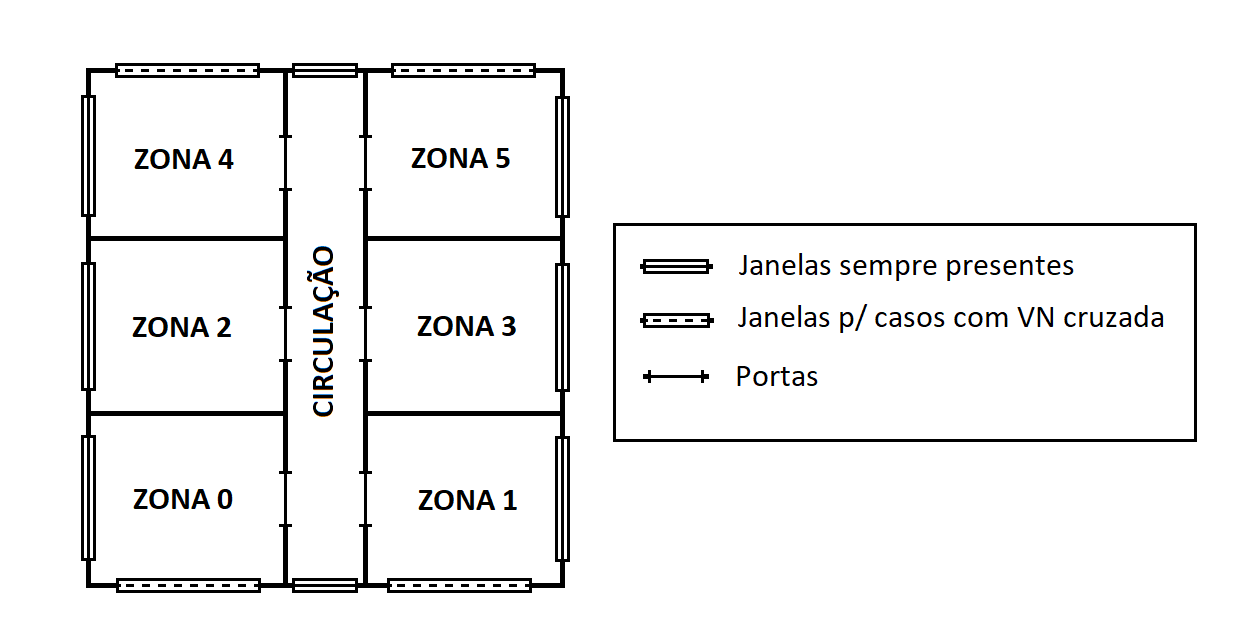
\includegraphics[width=1\linewidth]{img/croqui_07-11.png}
			\label{fig:croqui}
%			\begin{flushleft}
%				Fonte: o autor.
%			\end{flushleft}
		\end{figure}
		
		
		A partir da tipologia base, foi possível definir diferentes proporções geométricas, levando-se em consideração a largura e profundidade da edificação, assim como o pé-direito. Também foram parametrizadas a altura do pavimento e a orientação solar da edificação.
		Devido a limitações na obtenção dos coeficientes de pressão (Cp) para as faces externas da edificação, as edificações foram modeladas com pavimentos de forma retangular.
		
		A parametrização nas propriedades termofísicas das paredes e vidros permitiu a consideração de diferentes materiais construtivos, possibilitando a descrição de uma quantidade significativa do universo de casos aplicáveis às edificações de escritórios consideradas. %Foram parametrizadas a transmitância térmica, capacidade térmica e absortância.
		
		Para considerar o uso de ventilação natural (VN), é fundamental a modelagem das trocas de ar nos escritórios. A modelagem da VN nas simulações foi realizada com os objetos do \textit{AirflowNetwork} (AFN) do EnergyPlus \cite{EnergyPlus2018}.
		Para possibilitar trocas de ar, elementos de ligação do AFN foram modelados em todas as zonas térmicas.
		Todas as aberturas foram modeladas utilizando-se o objeto \textit{AirflowNetwork:MultiZone:Component:DetailedOpening}.
		Cada sala foi modelada com uma porta, voltada para a circulação.
		Na circulação, além das portas das salas, duas janelas foram modeladas, uma em cada extremidade. 
		Salas com apenas uma fachada foram modeladas com uma janela; salas com duas fachadas foram modeladas com uma ou duas janelas. Isso possibilitou explorar casos com diferentes configurações de exposição das superfícies, considerando-se VN unilateral e cruzada.		
		As dimensões das janelas das salas foram parametrizadas de acordo com o percentual de abertura da fachada (PAF), permitindo diferentes frações de abertura para representar diferentes modelos de janela encontrados nas edificações de escritórios existentes no banco de dados.
		%Além da área da abertura ter influência direta nas trocas de ar das zonas, a altura também pode ter influência devido à força de empuxo causada pelas diferenças de densidade do ar. Devido a isso, a altura da janela também foi parametrizada.
%		Para o vidro das janelas considerou-se diferentes valores para o fator solar.
%		\subsection{Ventilação natural no modelo preliminar}
		O controle das janelas foi estabelecido pela diferença de temperatura entre o ar externo e o ar da zona.
		As trocas de ar nas portas foram modeladas apenas por frestas, por considerar-se que portas de escritórios não ficam abertas normalmente.  % MELHORAR!!!
		Os coeficientes de pressão nos nós externos à edificação foram definidos através da base de dados da Universidade Politécnica de Tóquio (TPU) \cite{TPU2018}, e para cada janela foi utilizado o valor médio dos pontos disponíveis para sua área na fachada. No o exemplo da Figura \ref{fig:tpuwindows}, considerando-se uma edificação com proporções B:L:H, e um pavimento na altura h, o Cp da janela A seria igual a média dos valores disponíveis para os pontos vermelhos, o Cp da janela B seria igual a média dos valores dos pontos verdes, e assim por diante.
%		A altura dos pontos a serem utilizadas foi escolhida de acordo com a altura definida para o pavimento simulado e  a altura do pédireito em relação às proporções do edifício.
		
		\begin{figure}[h]
			\centering
			\caption{Exemplo de como os Cp’s foram considerados}
			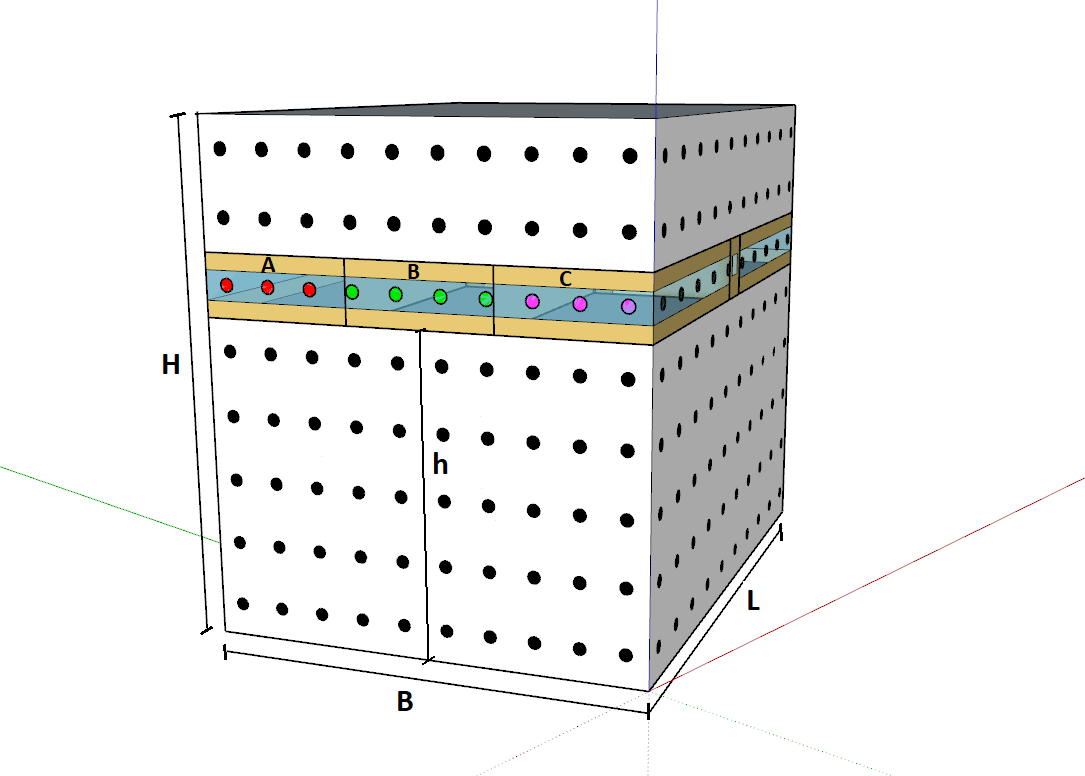
\includegraphics[width=1\linewidth]{img/ex_TPU_h.png}
			\label{fig:tpuwindows}
%			\begin{flushleft}
%				Fonte: \citeauthoronline{TPU2018} \cite{TPU2018}, adaptado pelo autor.
%			\end{flushleft}
		\end{figure}
		
		
		\subsection{Simulações simplificadas}
		
		Nesta etapa do método, buscou-se simplificar o modelo de escritório desenvolvido no EnergyPlus, atentando-se às limitações relacionadas à simplificação do modelo.
		O objetivo de gerar um metamodelo por meio de redes neurais artificiais (RNA) para se obter a EHF faz com que se busque parametrizar ao máximo as simulações no EnergyPlus.
		Essa parametrização pode facilitar o desenvolvimento de amostras para a pesquisa, assim como garantir uma relação mais direta dos parâmetros de entrada com os dados de saída. 
		Dentre as simplificações consideradas, estão:
		
		\begin{itemize}
		\item cálculo do Cp através do método analítico, em vez dos valores obtidos por medições em túnel de vento pela TPU;
		\item representação dos materiais da envoltória através de duas camadas: uma camada representando a capacidade térmica, e uma camada para regular a transmitância;  %(concreto)  (objeto Material:NoMass)
		\item modelagem da zona que representa apenas um escritório, sem modelar as demais zonas térmicas da edificação. Para isso, são definidas as condições de contorno relacionadas às faces da zona correspondentes a paredes adjacentes à edificação;
		\item definição de um coeficiente de fluxo mássico de ar relacionado à infiltração de ar pela porta, e do valor do Cp relacionado a essa porta, que no modelo de uma zona está voltada para o ambiente externo, e não para a circulação.
		\end{itemize}
		
		O impacto nos resultados das simulações foram verificados para cada uma das simplificações mencionadas, a partir da análise de diversos casos amostrados pelo método de amostragem do hipercubo latino (LHS). O tamanho das amostras foi definido em relação ao tempo disponível para executar as simulações.
		Finalmente, foi definida a forma mais adequada de se simplificar o modelo, assim como a margem de erro que espera-se encontrar ao assumir tais simplificações.
		A seguir, cada uma dessas etapas é descrita.
		
%		Nem todos os parâmetros foram variados em todas as etapas deste processo. Optou-se por variar apenas os parâmetros que pudessem influenciar os resultados relacionados a cada análise. Quando não variados, os parâmtros tiveram seus valores fixados de acordo com a Tabela \ref{table:paramfix}.
%		
%		\begin{table}[h]
%			\centering
%			\caption{Parâmetros fixados na validação do modelo analítico para o cálculo do Cp.}
%			\label{table:paramfix}
%			\begin{tabular}{|c |c |}
%				\hline
%				\textbf{Parâmetro} & \textbf{Valor adotado} \\
%				\hline
%				Altura do pavimento & 15 m \\
%				\hline
%				Fator solar do vidro & 0,87 \\
%				\hline
%				Fator de abertura da janela & 1,0 \\
%				\hline
%				Capacidade térmica da parede & 155 kJ/m$^2$K \\
%				\hline
%				Absortância da parede & 0,5 \\
%				\hline 
%				Ângulo de sombreamento & 0 graus \\
%				\hline 
%			\end{tabular}
%			\begin{flushleft}
%				Fonte: o autor.
%			\end{flushleft}				
%		\end{table}
%		
%		
		\subsubsection{Cálculo do coeficiente de pressão pelo método analítico}
		
		O EnergyPlus, através do AFN, possui uma opção para calcular automaticamente os Cp's para as simulações.
		Quando essa opção é escolhida o programa gera apenas um Cp por fachada da edificação, e os valores podem ser obtidos por dois algorítimos diferentes: no caso de edificações altas (\textit{highrise}), utiliza-se o modelo de \citeauthoronline{Atkins} \cite{Atkins}; no caso de edificações baixas (\textit{lowrise}), utiliza-se o modelo de \citeauthoronline{SwamiChandra} \cite{SwamiChandra}.
		Enquanto que pelo método analítico (MA) os Cp's podem ser obtidos para quaisquer razões entre as dimensões das fachadas da edificação, os valores medidos em túnel de vento pela TPU são fornecidos para edificações com proporções entre largura, profundida e altura específicas.
		Os valores de Cp para o tipo de edificação abordada neste estudo são disponibilizados pela TPU para 25 geometrias diferentes, das quais 13 são para edificações \textit{highrise}, e 12 são para edificações \textit{lowrise}.
		
		Para verificar o quanto a fonte escolhida na definição dos Cp's influencia nos resultados das simulações, inicialmente verificou-se as diferenças entre os valores dos Cp's das medições em túnel de vento (fornecidos pela TPU), e os valores dos Cp's obtidos pelo MA (algorítimos do EnergyPlus). Para cada uma das 25 geometrias disponíveis, calculou-se a diferença entre os Cp's, de acordo com a Equação \ref{eq:Cpdiff}.
		
		\begin{equation}
		\label{eq:Cpdiff}
		\overline{\Delta}_{Cp} = \frac{\sum_{i=1}^{4}{\sum_{j=0}^{11}{|\overline{Cp}^{TPU}_{f_i,\alpha_j} - Cp^{MA}_{f_i,\alpha_j}}|}}{48}
		\end{equation}
		
		Onde:
		
		$\overline{\Delta}_{Cp}$ é igual à diferença absoluta média entre os valores dos Cp's obtidos pela base da TPU e obtidos pelo MA;
		
		$\overline{Cp}^{TPU}_{f_i,\alpha_j}$ é igual ao valor médio dos Cp's disponibilizados pela base de dados da TPU para a fachada $i$ de uma edificação, para o ângulo de incidência do vento igual a $\alpha_j$;
		
		$Cp^{MA}_{f_i,\alpha_j}$ é igual ao Cp calculado pelo MA para a fachada de uma edificação com proporções iguais às da fachada $i$, para o ângulo de incidência do vento igual a $\alpha_j$;
		
		$f_i$ é a fachada $i$ da edificação avaliada;
		
		$\alpha_j$ é o ângulo de incidência do vento  sobre a fachada, em graus, e tem valor igual a $30 \cdot j$.		
		%		$\alpha_j$ é o ângulo de incidência do vento considerado sobre a fachada, que varia de 0 a 330 graus, com intervalos de 30 graus;
		\\
		
%		Cada Cp médio ($Cp_{TPU,i,j}$), medido pela TPU em um ponto $j$ de uma fachada $i$, teve um Cp correspondente calculado pelo método analítico ($Cp_{ANALITICO, i}$), para a mesma fachada $i$. Essa subtração foi efetuada para os diferentes ângulos ($\alpha$) disponíveis na base da TPU.
%		As diferenças entre os valores dos Cp's foram calculadas obtendo-se o Cp pelo método analítico para cada fachada, de cada geometria disponível pela TPU, e subtraindo-se o valor do Cp calculado pelos valores disponibilizados pela base da TPU para a sua fachada correspondente (Equação \ref{eq:Cpdiff}).

		A partir dessas diferenças entre os valores dos Cp's ($\overline{\Delta}_{Cp}$), escolheu-se a geometria com a maior diferença absoluta média como modelo base na análise da influência nos resultados das simulações no EnergyPlus.
		Esta análise foi conduzida gerando-se uma amostra de 1.000 casos pelo LHS.
		Os parâmetros variados e seus limites mínimos e máximos foram definidos pela metodologia do item \ref{subsec:par}, com exceção da razão entre a largura e profundidade das zonas e a altura do pavimento em relação ao solo.
		A razão entre a largura e profundidade das zonas teve que ser alterada de acordo com a variação da área das salas, para se ajustar à geometria da edificação definida como modelo base da análise.
		A altura do pavimento em relação ao solo também foi limitada pelas proporções da geometria escolhida para o modelo base.
		Vale destacar que a base da TPU permite a obtenção de diferentes Cp's para diferentes janelas de uma mesma fachada, enquanto que nas simulações baseadas no MA, utiliza-se apenas um valor de Cp por fachada, devido à limitação do método. 
		Para cada caso da amostra gerada, foram simulados um modelo com Cp’s baseados no MA, e um modelo com Cp’s baseados na base da TPU (túnel de vento).
		Assim, as trocas de ar por hora (ACH) e a EHF foram comparadas entre as simulações.
		%		com Cp's medidos em túnel de vento pela TPU, e simulações com Cp's obtidos pelos métodos analíticos padrão do EnergyPlus.
				
%		Para cada uma dessas geometrias disponíveis, valores de Cp são disponibilizados para diversos pontos na fachada da edificação, de acordo com a Figura \ref{fig:tpupoints}.
%		
%		\begin{figure}[h]
%			\centering
%			\caption{Exemplo do posicionamento dos pontos com valores de Cp na fachada}
%			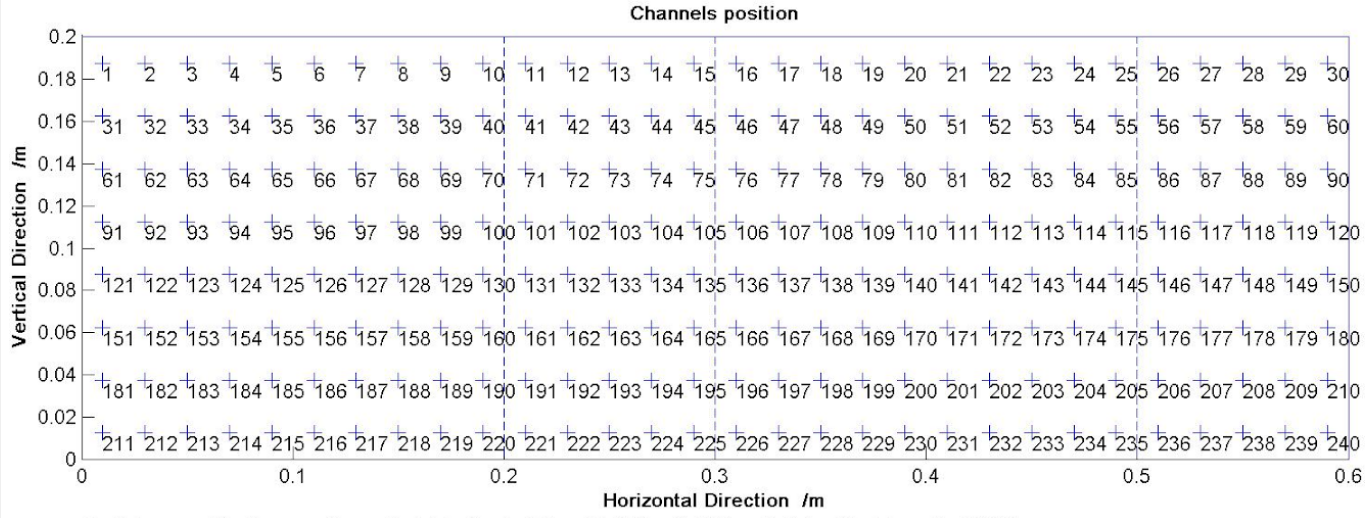
\includegraphics[width=1\linewidth]{img/tpu_points.png}
%			\label{fig:tpupoints}
%			\begin{flushleft}
%				Fonte: \citeauthoronline{TPU2018} \cite{TPU2018}, adaptado pelo autor.
%			\end{flushleft}
%		\end{figure}					
		
		\subsubsection{Representação da envoltória com duas camadas}
		
		Para possibilitar a parametrização contínua e independente das propriedades termofísicas da envoltória, considerou-se a utilização de uma parede com propriedades equivalentes, modelada com uma camada de concreto, para representar a capacidade térmica, e uma camada modelada com o objeto \textit{Material:NoMass}, para regular a transmitância (Figura \ref{fig:parede_eq}).
		
		\begin{figure}[h]
			\centering
			\caption{Parede equivalente}
			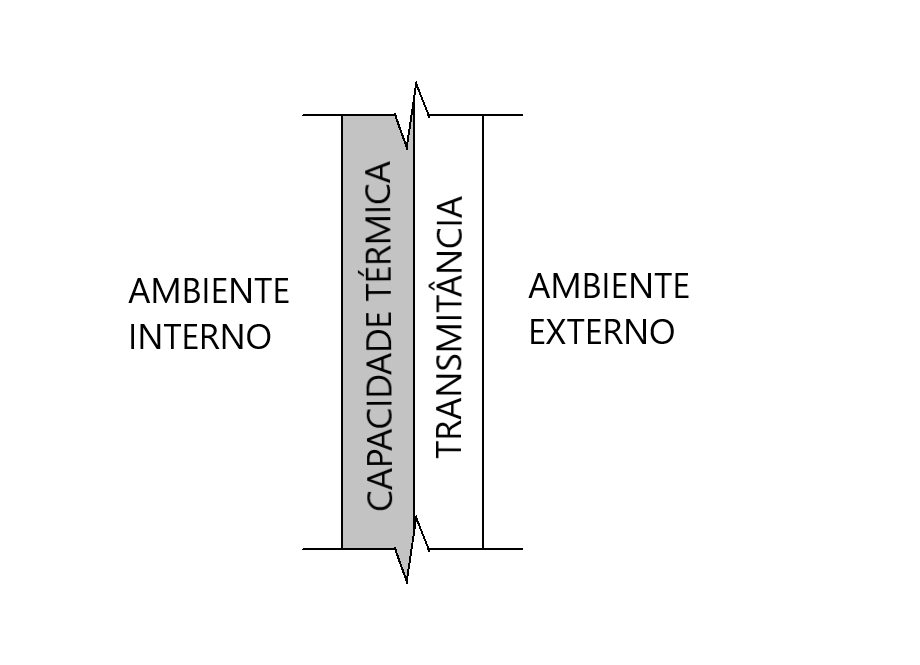
\includegraphics[width=1\linewidth]{img/parede_eq.png}
			\label{fig:parede_eq}
		\end{figure}
	
		A validação da modelagem simplificada da parede foi feita para dois tipos de paredes referência:
		
		\begin{itemize}
%			\item parede de concreto;
			\item parede de gesso com lã de rocha;
			\item parede de alvenaria e reboco.
		\end{itemize}
		
		Como a modelagem da parede de alvenaria possui uma camada de ar no meio da parede, avaliou-se a possibilidade de considerar apenas a metade interna desta parede referência para definir a capacidade térmica de sua parede equivalente. Essa consideração parte do pressuposto de que a camada interna de ar faria com que a inércia térmica da metade exterior da parede não influenciasse consideravelmente a zona térmica analisada.
		
		Para validar essa simplificação, gerou-se uma amostra utilizando LHS, com 100 casos.
		Os parâmetros variados e seus limites mínimos e máximos foram definidos pela metodologia do item \ref{subsec:par}, com exceção da transmitância e capacidade térmica da parede.  % os parâmetros relacionados com a propriedades termofísicas da parede.	% e a absortância????
%		O modelo preliminar sofreu variação dos seguintes parâmetros: área, razão entre largura e profundidade da zona, pé-direito, azimute, absortância, PAF, taxa de ocupação. Os demais parâmtros foram fixados de acordo com a Tabela \ref{table:paramfix}.
		Cada caso da amostra foi simulado com os dois tipos de paredes diferentes, e suas paredes equivalentes. No caso da parede de alvenaria, dois modelos de parede equivalente foram desenvolvidos: considerando a capacidade térmica total da parede, e considerado apenas metade da capacidade térmica.
		A partir dos resultados, observou-se a diferença média entre as temperaturas operativas das zonas simuladas com as paredes referências em relação às simulações com as respectivas paredes equivalentes. O mesmo foi feito comparando-se a EHF.
		
		\subsubsection{Condição de contorno das paredes adjacentes à edificação}
		
		Simular apenas uma zona térmica, em vez de um edifício inteiro, ou um pavimento com diversas zonas, possibilita a simulação de casos diversos em menor tempo.
		A partir dessa premissa, foi desenvolvido um modelo com apenas uma zona térmica (Figura \ref{fig:singlezone}).
		
		\begin{figure}[h]
			\centering
			\caption{Modelo de uma zona}
			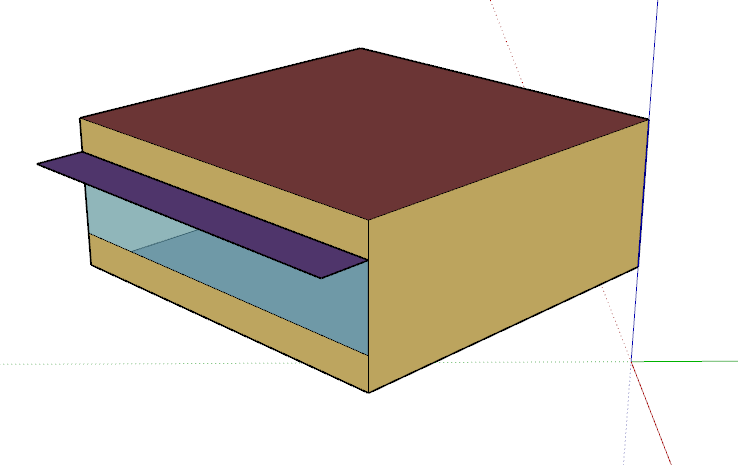
\includegraphics[width=1\linewidth]{img/model.PNG}
			\label{fig:singlezone}
		\end{figure}
		
		Para modelar essa zona, considerou-se as paredes correspondentes a superfícies voltadas para outros escritórios como adiabáticas. A superfície que representa a parede voltada para a circulação foi testada com duas condições de contorno: 1) como adiabática, e 2) como \textit{outdoors}, sem incidência de vento ou sol (Figura \ref{fig:adiabatic_outdoors}).	
		A consideração do uso da condição \textit{outdoors} foi pela hipótese de que, sem a radiação solar direta e sem o aumento de convecção causada pelo vento, a temperatura do ar da zona da circulação (por não ter cargas internas consideráveis) poderia se manter mais próxima à temperatura do ar externo do que às das zonas das salas de escritórios.
		
		\begin{figure}[h]
			\centering
			\caption{Modelagem com parede adiabática e \textit{outdoors}}
			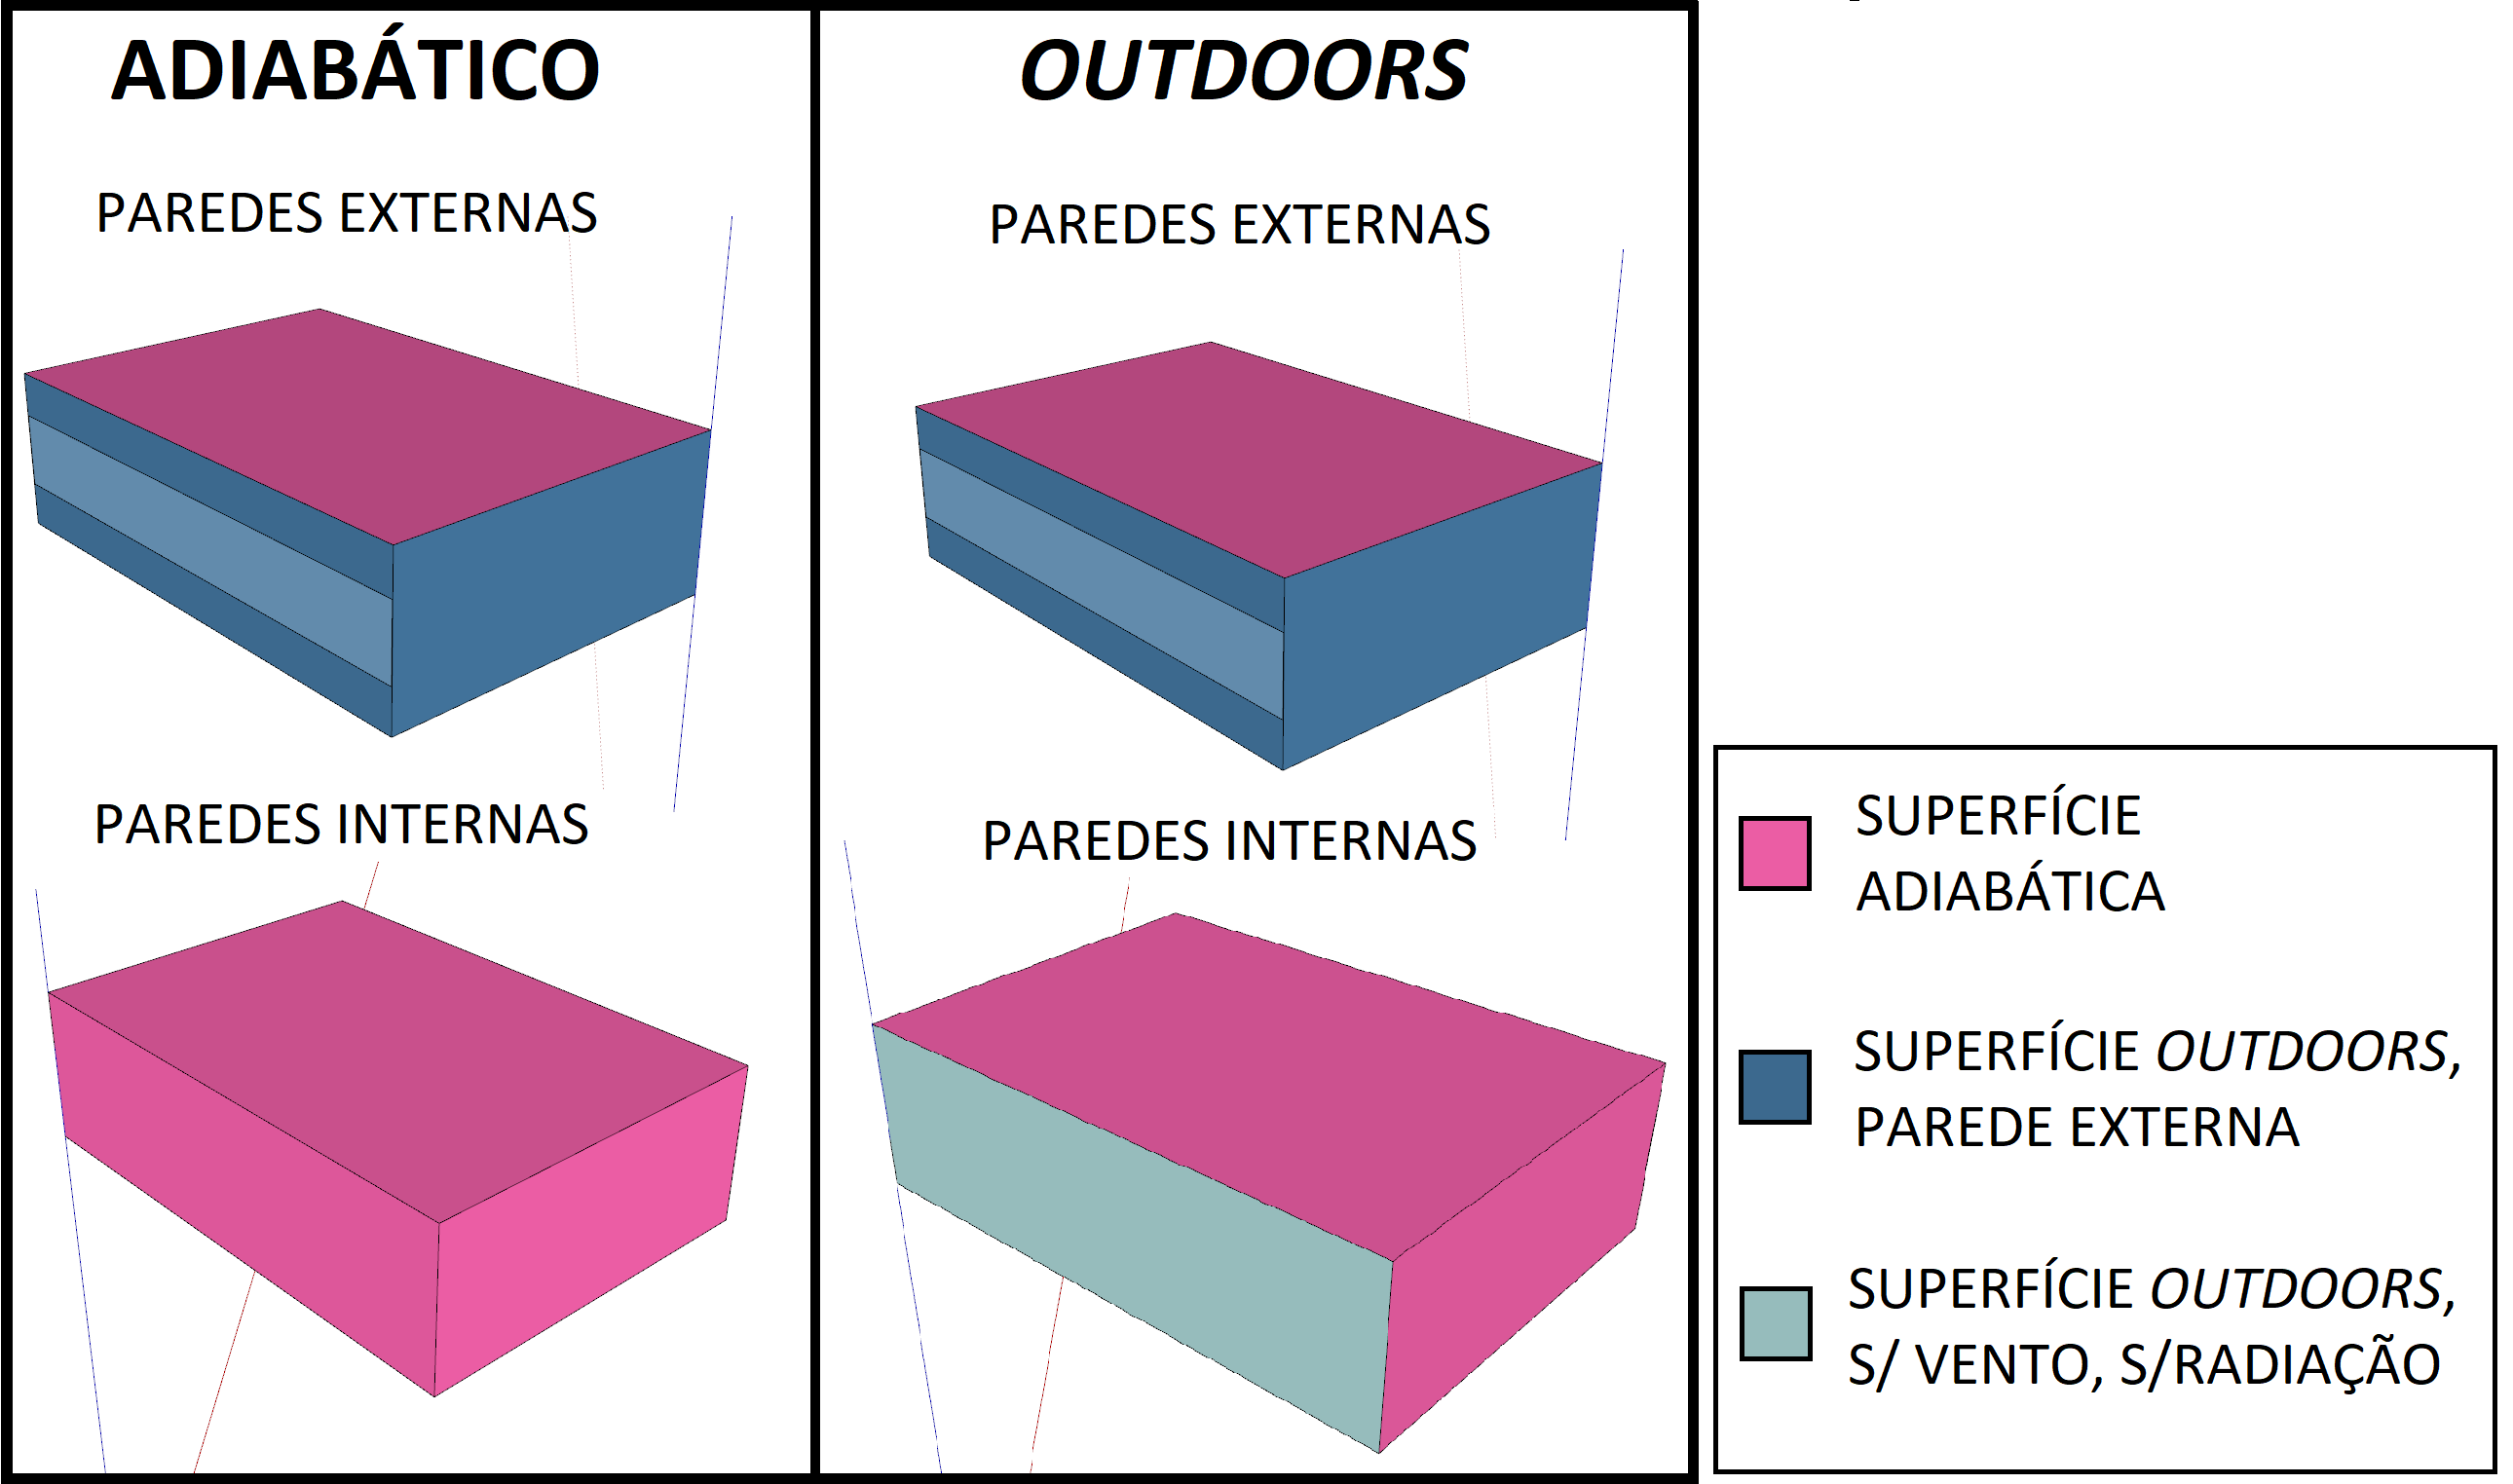
\includegraphics[width=1\linewidth]{img/adiabatic_outdoors.png}
			\label{fig:adiabatic_outdoors}
		\end{figure}
	
		
		A modelagem da ventilação natural sofre um impacto significativo quando o escritório é modelado como apenas uma zona térmica.
		Esse impacto é devido à forma como a rede de fluxo de ar é montada. No caso do modelo referência, a porta é voltada para a circulação, enquanto que no caso de uma única zona térmica, a porta desta zona é voltada para o ambiente externo. 
		Além disso, não é possível modelar uma porta em uma parede adiabática. Para não deixar a diferença na ventilação natural influenciar as análises comparativas entre as simulações, a ventilação natural não foi modelada para esta etapa.
		Em vez disso, as simulações foram desenvolvidas com uma taxa de infiltração de ar constante durante a ocupação. O valor escolhido para a taxa de renovação de ar foi igual ao valor médio das ACH obtido na etapa da comparação entre os Cp's, que é igual a 30 ACH.
		
		A amostra gerada pelo LHS nesta etapa foi de 100 casos.
		Os parâmetros variados e seus limites mínimos e máximos foram definidos pela metodologia do item \ref{subsec:par}.
		Para cada caso, além da referência, seis modelos de uma zona foram simulados, correspondendo a cada uma das zonas do modelo referência.
		Para validar o uso de diferentes condições de contorno, comparou-se os resultados de EHF e temperaturas operativas das simulações de uma zona com as simulações referência.
		A condição de contorno com menores diferenças médias absolutas, de temperatura operativa e EHF, foi escolhida para se conduzir as simulações simplificadas.
		
		\subsubsection{Modelagem da ventilação natural na simulação simplificada}
		
		A modelagem da ventilação natural na simulação simplificada deve ser adaptada para se ter resultados correspondentes ao esperado em relação à simulação referência, pois enquanto a rede de fluxo de ar na simulação referência é modelada de acordo com a Figura \ref{fig:AFN_ref}, na simulação simplificada essa rede é modelada de acordo com a Figura \ref{fig:AFN_sz}.	
		
		\begin{figure}[h]
			\centering
			\caption{Rede de fluxo de ar na simulação referência}
				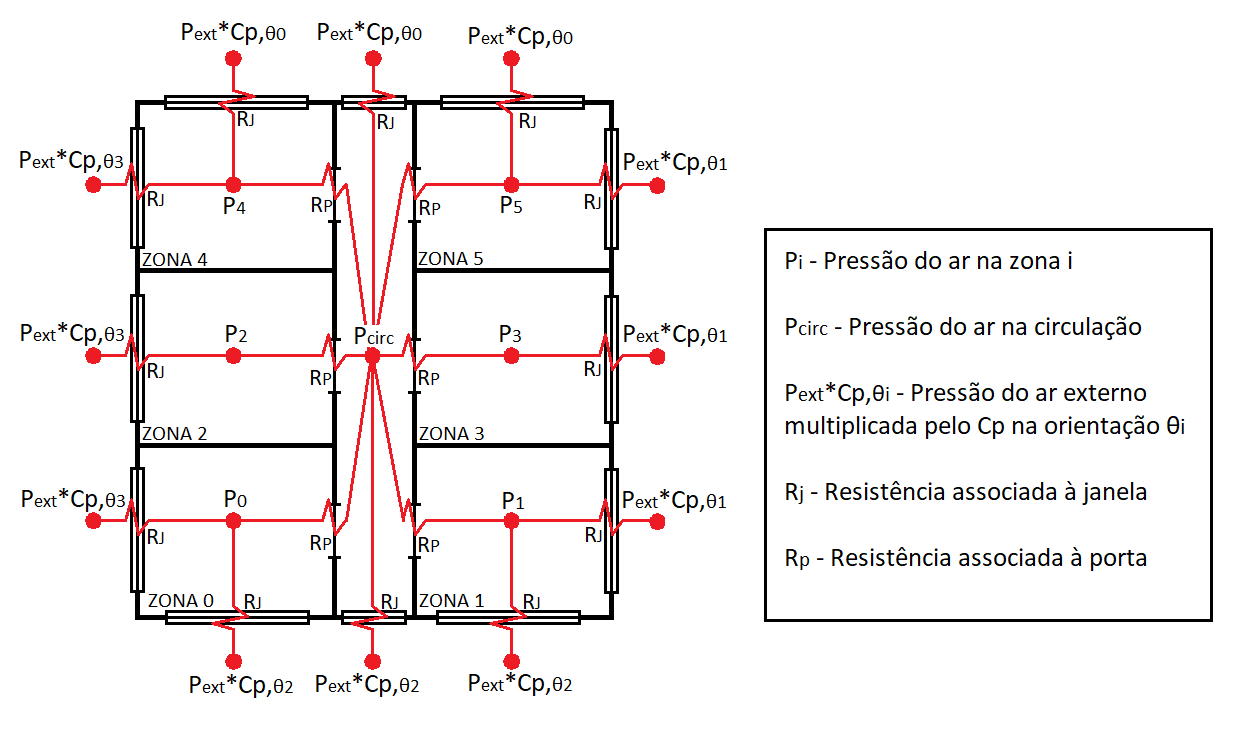
\includegraphics[width=1\linewidth]{img/AFN_ref.png}
				\label{fig:AFN_ref}
		\end{figure}	
		
		\begin{figure}[h]
		\centering
		\caption{Rede de fluxo de ar na simulação simplificada}
			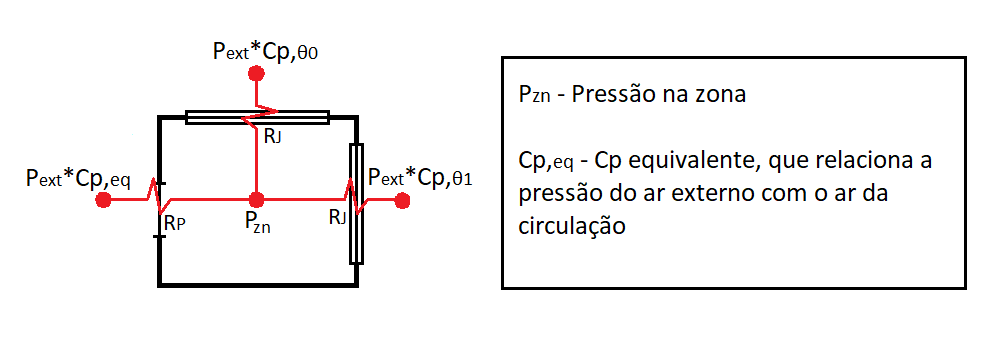
\includegraphics[width=1\linewidth]{img/AFN_sz.png}
			\label{fig:AFN_sz}
		\end{figure}
%		As limitações desta adaptação e as formas de contorná-las serão explicadas neste item.
		
		A proposta para contornar esse problema foi desenvolvida a partir da hipótese de que, na simulação simplificada, seria possível criar um Cp associado à porta ($Cp_{eq}$), capaz de descrever as diferenças de pressão de ar entre a circulação e a sala.  % , para cada ângulo de vento.
		
		Quando o objeto \textit{AirflowNetwork:MultiZone:Component: DetailedOpening} é utilizado, o cálculo do fluxo de ar entre dois pontos é feito pela Equação \ref{eq:AFEDOP_opened}, se a porta/janela está aberta, ou pela Equação \ref{eq:AFEDOP_closed}, que é utilizada para calcular a infiltração de ar quando a abertura está fechada.
		
		\begin{equation}
		\label{eq:AFEDOP_opened}
		\dot{m}_{i,j} = C_d \Theta 	\int_{z=0}^{z=H} \sqrt{2 \rho (P_{i(z)} - P_{j(z)})} W d_z 
		\end{equation}
		
		\begin{equation}
		\label{eq:AFEDOP_closed}
		\begin{split}
		\dot{n}_{i,j} = C_q [2\int_{z=0}^{z=H} {(P_{i(z)} - P_{j(z)})}^{exp} d_z + \\ W{(P_{i(0)} - P_{j(0)})}^{exp} + W{(P_{i(H)} - P_{j(H)})}^{exp}]
		\end{split}
		\end{equation}
		
		Onde:
		
		$\dot{m}_{i,j}$ é o fluxo de ar entre os pontos $i$ e $j$, quando a porta/janela está aberta;
		
		$C_d$ é o coeficiente de descarga da abertura;
		
		$\Theta$ é a fração de abertura;
		
		$H$ é a altura da abertura;
		
		$\rho$ é a densidade do ar;
		
		$P_{i(z)}$ é a pressão de ar no ponto $i$, altura $z$;
		
		$W$ é a largura da abertura;
		
		$\dot{n}_{i,j}$ é o fluxo de ar entre os pontos $i$ e $j$, quando a porta/janela está fechada;
		
		$C_q$ é o coeficiente de fluxo mássico de ar da abertura;
		
		$exp$ é o expoente de fluxo de massa de ar.
		\\
		
		As seguintes condições de contorno foram criadas para facilitar o cálculo do $Cp_{eq}$:
		\begin{itemize}			 
			\item o valor do $exp$ foi definido como 0,5;
			\item o valor de $\rho$ foi definido sempre como 1,200 kg/m$^3$;
			\item os fluxos de ar foram considerados como unidimensionais, portanto os valores de $P$ não variaram com o a altura ($z$);
			\item O valor do $Cp_{eq}$ foi definido assumindo-se que as janelas estariam com sua máxima fração de abertura ($\Theta$).
		\end{itemize}
		
		Em cada \textit{timestep}, a soma dos fluxos de ar que entram e saem de uma zona $i$ é igual a zero. Assumindo-se as condições de contorno descritas, a pressão de ar em cada zona térmica pode ser estimada pela Equação \ref{eq:P}. Dessa forma é possível encontrar a relação entre as pressões de ar de todas as zonas da simulação de referência.
		
		\begin{equation}\label{eq:P}
		%\resizebox{\linewidth}{!}{
		\begin{split}
		P_{zn} = \frac{\sum_{i=1}^{N_P}{P_{i} (C_q L_i)^2} +  %\\
		\sum_{j=1}^{N_J}{P_{ext} C_{p,j} 2 \rho (C_{d} \Theta_j A_j)^2 }}
		{\sum_{i=1}^{N_P}{(C_q L_i)^2} +  %\\
			\sum_{j=1}^{N_J}{2 \rho (C_{d} \Theta_j A_j)^2 }}
		\end{split}
		%}
		\end{equation}
		
		Onde:
		
		$P_{zn}$ é a pressão do ar na zona analisada;
		
		$N_P$ é igual ao número de portas que se conectam à zona;
		
		$P_i$ é a pressão de ar na zona ligada pela porta $i$;
		
		$L_i$ é igual ao perímetro da porta $i$;
		
		$N_J$ é igual ao número de janelas que se conectam à zona;
		
		$P_{ext}$ é a pressão do ar no ambiente externo;
		
		$C_{p,j}$ é o Cp na superfície da janela $j$;
		
		$A_j$ é igual à área da janela $j$.
		\\
		
		Finalmente, os Cp's equivalentes ($Cp_{eq}$) foram definidos calculando-se a relação entre a pressão de ar na zona da circulação e a pressão do ar no ambiente externo, para cada direção angular do vento, de acordo com a Equação \ref{eq:Cpeq}.
		
		\begin{equation}\label{eq:Cpeq}
		Cp_{eq,\alpha} = \frac{P_{circ}}{P_{ext}}
		\end{equation}
		
		Onde:
		
		$P_{circ}$ é a pressão de ar na circulação;
		
		$Cp_{eq,\alpha}$ é igual ao Cp equivalente na abertura da porta, para um ângulo de vento $\alpha$.
		\\
		
		Outra limitação relacionada à VN na simulação simplificada é o fato de que o AFN do EnergyPlus não permite modelar aberturas ou qualquer tipo de infiltração de ar em superfícies adiabáticas. Para contornar esse problema, no caso de se modelar uma parede voltada para a circulação como adiabática, é possível associar a infiltração referente à porta a uma outra superfície da zona.  %  que esteja voltada para o ambiente externo 
		Isso se faz possível no momento em que se calcula diretamente os coeficientes de pressão (Cp's) dos nós relacionados às aberturas da zona.
		Desta forma define-se o Cp para uma superfície (seja janela ou parede), considerando-se qualquer orientação desejada, e não necessariamente a orientação definida para esta superfície pela geometria do modelo.		
		A modelagem do fluxo de ar pelas portas dos escritórios nas simulações simplificadas foi desenvolvida com o objeto \textit{AirflowNetwork:MultiZone:Surface:Crack}. O motivo para se utilizar este objeto é porque este é um objeto que pode ser associado a qualquer tipo de superfície. Portanto, o objeto do \textit{crack} foi associado sempre à parede externa oposta à parede que estaria voltada para a circulação, como apresentado na Figura \ref{fig:AFN_crack}.
		
		\begin{figure}[h]
			\centering
			\caption{Solução para infiltração de ar entre a zona e a circulação}
			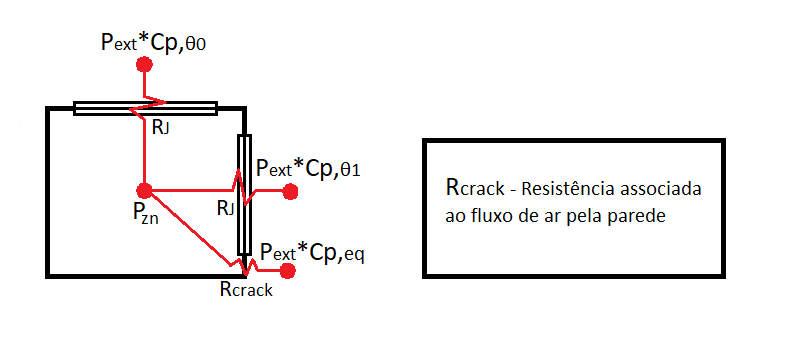
\includegraphics[width=1\linewidth]{img/AFN_crack.png}
			\label{fig:AFN_crack}
		\end{figure}	
					
		Devido a essas considerações, a validação nesta etapa foi conduzida para duas condições: utilizando-se o Cp calculado diretamente pelo método analítico, e utilizando-se o $Cp_{eq}$.		
		Estas análises foram conduzidas considerando-se diferentes valores de coeficiente de fluxo mássico de ar para o \textit{crack}, para ajustar o valor mais adequado à taxa de infiltração que se obtém no modelo referência. Os valores considerados foram: 0,10; 0,30; 0,40; 0,45; 0,50; 0,55; 0,6; 0,7; 0,80; e 0,90 kg/s em 1 Pa.
		Uma amostra de 200 casos foi gerada por LHS.
		Os parâmetros variados e seus limites mínimos e máximos foram definidos pela metodologia do item \ref{subsec:par}.
		Para cada caso, gerou-se uma simulação referência, mais dez simulações simplificadas. Essas dez simulações devem-se a consideração dos dois métodos para se obter os Cp's, mais os dez valores de coeficiente de fluxo mássico de ar analisados. As comparações foram efetuadas observando-se os resultados de ACH e EHF. 
		%Como as taxas de infiltração são influenciadas pela temperatura do ar, as comparações com os modelos referências foram feitas considerando-se diferentes faixas de temperatura.
		
		\section{Análise de sensibilidade}
		
		Após definir como seriam gerados os modelos para as simulações simplificadas, uma análise de sensibilidade (AS) foi aplicada. Através da AS, a influência dos diferentes dados de entrada variados nas simulações foi avaliada. Com base nos resultados da AS, parâmetros não relevantes nos resultados de temperatura operativa e, consequentemente, fração de horas de desconforto por calor (EHF), foram determinados com valores fixos.
		
		O método de \citeauthoronline{Sobol1993} \cite{Sobol1993} foi utilizado para a AS, pois permite a identificação de parâmetros influentes, mesmo para casos onde a relação entre as entradas e saídas dos modelos são não-monotônicas e apresentam efeitos colineares.
		
		A AS foi aplicada por meio de programação, utilizando-se a biblioteca \textit{SALib} \cite{Herman2017}, escrita na linguagem \textit{Python} \cite{Python}.
		Os casos simulados para conduzir a AS foram amostrados pelo método de amostragem específico da AS de Sobol, pelo qual gerou-se uma amostra de 99.978 casos.
		Os parâmetros variados e seus limites mínimos e máximos foram definidos pela metodologia do item \ref{subsec:par}. 
		%, que gera uma sequência quasi-randômica de baixa discrepância.é uma é feita a partir de uma amostra desenevolvida específica para essa análise é definida pelo próprio método, pela qual gerou-se 99.978 casos.		
		A partir dos dados de entrada de cada caso, e dos valores de EHF's resultantes das simulações termoenergéticas, obteve-se índices de sensibilidade para análise de 1ª ordem, 2ª ordem, e total.
		
		\section{Desenvolvimento do metamodelo}
		
		O metamodelo foi desenvolvido por meio de redes neurais artificiais (RNA).		
		A maneira como se descreve as variáveis de entrada dos modelos simulados para o metamodelo a ser desenvolvido pode influenciar na sua precisão e na representação adequada dos fenômenos termofísicos.
		Portanto, no processo de definição das variáveis de entrada do metamodelo, busca-se a melhor forma de descrever as diversas características das zonas térmicas.
		Esse é um processo iterativo, que envolve diferentes variáveis, utilizando-se às vezes transformações, normalizações e funções destas. 
		É importante também observar os hiper-parâmetros (parâmetros relacionados ao processo de aprendizagem automática) escolhidos no desenvolvimento da RNA. 
		A precisão dos resultados obtidos pela RNA pode depender do número de nós, número de camadas, taxa de aprendizagem, número de iterações, assim como outros parâmetros definidos durante o processo de treinamento. 
		
		Ao longo do processo de desenvolvimento do metamodelo, RNA's com diferentes configurações foram testadas, utilizando-se diferentes maneiras de descrever as variáveis de entrada, e diferentes combinações de hiper-parâmetros.
		A base de dados utilizada para o treinamento do metamodelo foi gerada a partir de 100.000 simulações, amostrados pelo método de amostragem de Sobol.
		A amostra utilizada para validação foi composta por 80.000 casos, geradas por LHS.
		% O motivo para se utilizar diferentes métodos de amostragem é para evitar qualquer enviesamento possivelmente relacionado ao método de amostragem.
		Em ambas as amostras, os parâmetros variados tiveram seus limites mínimos e máximos definidos de acordo com o item \ref{subsec:par}, com excessão daqueles parâmetros que tiveram seus valores determinados como fixos na etapa da AS.
		Os indicadores de precisão utilizados foram o erro absoluto médio e o erro absoluto do $95^{\circ}$ percentil.
		É comum se utilizar a raiz quadrada do erro quadrático médio (RMSE), ou o coeficiente de determinação (R$^2$) como indicadores de desempenho. Contudo, considerando-se que o dado de saída do metamodelo será uma fração (EHF) com valor entre zero e um, o erro absoluto já é consequentemente um erro relativo. Portanto, conclui-se que o erro absoluto médio, associado ao erro absoluto $95^{\circ}$ percentil, pode estimar de maneira mais adequada a imprecisão esperada para os resultados do metamodelo.
		
		A RNA com os melhores indicadores de precisão na etapa de treinamento foi escolhida para ter seu desempenho analisado com uma amostra de teste. 
		A amostra de teste foi utilizada para verificar o desempenho da RNA quando os valores dos parâmetros determinados como fixos na etapa da AS variam. Para isso, utilizou-se a mesma amostra gerada para etapa da AS, pois as simulações já estavam finalizadas, e os casos eram diferentes daqueles utilizados no desenvolvimento da RNA.
		Ao analisar os indicadores de precisão da RNA em relação às amostras de validação e de teste, o metamodelo final foi definido.

%\bibliographystyle{lib/abntex2-num}
%\bibliographystyle{lib/abntex2-alf}
\bibliography{citacoes}
	
\end{document}